\section{Code Struktur/Übersicht}
\label{sec:code-structure}
Das \currentauthor{David Piper und\\ Florian Grieskamp} Framework besteht hauptsächlich aus den vier Unterordnern \textit{bigtest}, \textit{external}, \textit{sacabench} und \textit{tests}. \par
Bigtests sind Tests auf sehr großen Texten.
Die Ausführung wird mit \termfont{make bigtest} gestartet und anschließend werden verschiedene große Textdateien geladen und lokal in dem Ordner external/datasets/ gespeichert. 
Die Dateien stammen von der Seite \termfont{dolomit.cs.uni-dortmund.de/} und umfassen unter anderem Quellcode, DNA und Auszüge von Wikipedia.
Ist der Download abgeschlossen, werden die SACAs mit diesen heruntergeladenen Textdateien ausgeführt und das Ergebnis auf Korrektheit überprüft. \par
Im Ordner external liegen neben diesen Texten auch verschiedene Bibliotheken, welche innerhalb des Projekts eingebunden werden.
Außerdem sind die Referenzimplementierungen der SACAs im Unterordner external/reference\_impls enthalten. 
Diese können vom Framework mit Hilfe von Wrappern verwendet werden, welche sich im Ordner sacabench befinden. \par
Der Ordner sacabench ist der Hauptbestandteil des Frameworks. 
In diesem befindet sich der Unterordner saca, welcher die Implementierungen der SACAs enthält. 
Zusätzlich befindet sich hier der Ordner external, in dem die zuvor beschriebenen Wrapper zur Einbindung der externen Referenzimplementierungen vorhanden sind. 
Alle SACAs enthalten die Wert \termfont{EXTRA\_SENTINELS}, \termfont{NAME} und \termfont{DESCRIPTION}. 
\termfont{EXTRA\_SENTINELS} bestimmt die Anzahl der zusätzlichen Sentinels, die von dem Framework vor Aufruf des Algorithmus an den zu verarbeitenden Text angehangen werden müssen. 
\termfont{NAME} und \termfont{DESCRIPTION} werden bei Aufruf von \termfont{sacabench list} ausgegeben. 
Zusätzlich stellt jeder SACA die Methode \termfont{construct\_sa} bereit, welche den Algorihtmus auf den übergebenene Text anwendet. 
Die Wrapper stellen diese Werte für die externen Referenzimplementierungen bereit.
Neben dem Ordner saca befindet sich der Ordner util. 
In diesem sind verschiedenen Hilfsfunktionen und -klassen implementiert, beispielsweise finden sich hier unterschiedliche Sortieralgorithmen, die von den SACAs verwendet werden. 
Zuletzt befindet sich hier die Datei sacabench.cpp, welche das CLI implementiert. 
Sie enthält die main-Funktion, welche die eingegebenen Parameter verarbeitet und die ausgewählten Algorithmen startet.\par
Der Ordner tests umfasst eine Menge von Testfällen, welche mit \termfont{make check} ausgeführt werden können. 
Neben den Tests für die einzelnen Util-Klassen und -Funktionen stellt die Datei saca.hpp viele verschiedene Testeingaben bereit, mit denen die Korrektheit der internen und externen SACAs überprüft werden kann. 
Anschließend wird das Ergebnis mit einem Referenz-SACA verglichen. 
Die Testeingaben, auf die die SACAs angewendet werden, umfassen verschiedene Sprachen und Zeichensätze, u.a. einen All-a-Text, Smileys, Kanji und Hieroglyphen.\par
Die Abbildung \ref{ordner_struktur} visualisiert die beschriebenen Bestandteile der Ordnerstruktur.

\begin{figure}[t!]
\centering
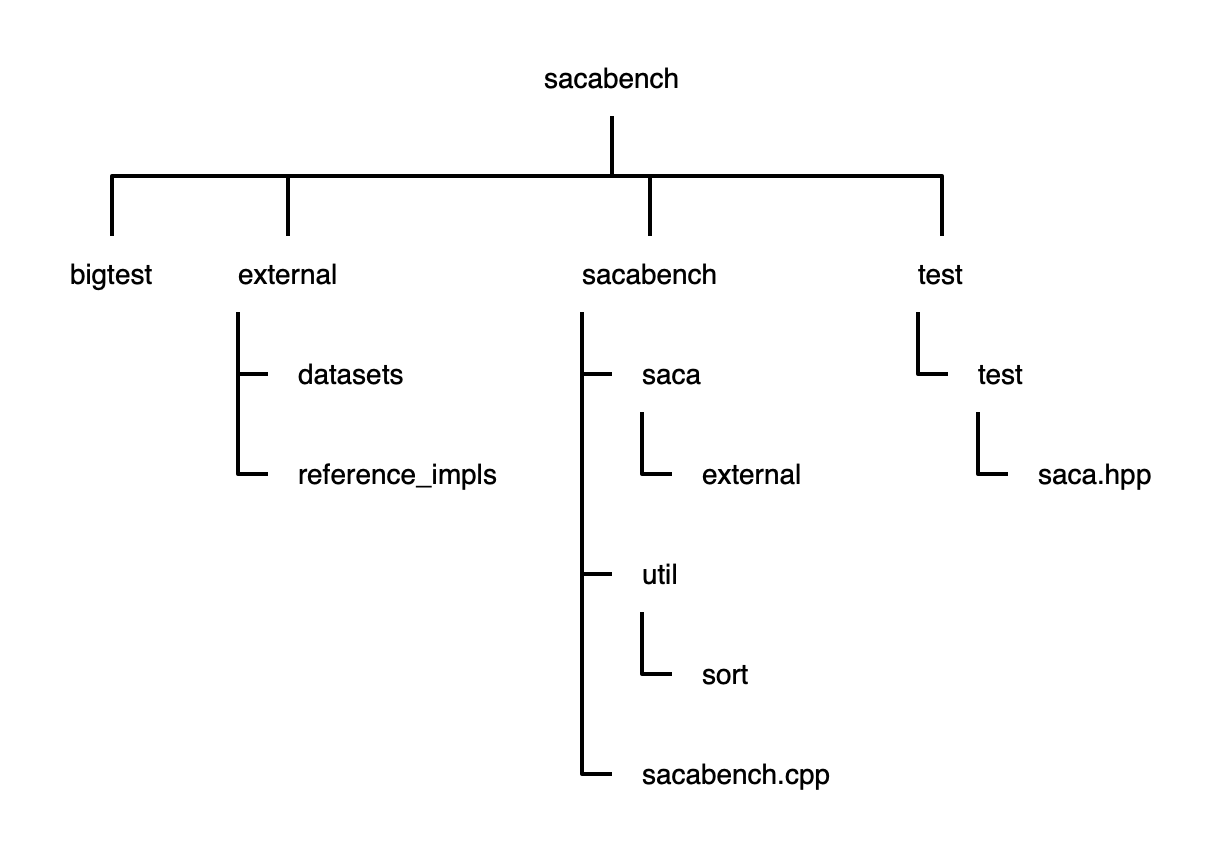
\includegraphics[width=\textwidth]{kapitel/3_framework/code_structure/ordner_struktur}
\caption[Ausschnitt der beschriebenen Ordnerstruktur.]{Ausschnitt der beschriebenen Ordnerstruktur.}
\label{ordner_struktur}
\end{figure}